\documentclass[11pt,a4paper]{article}

\usepackage[utf8]{inputenc}
\usepackage[T1]{fontenc}
\usepackage[spanish]{babel}
\usepackage{amsmath}
\usepackage{amsfonts}
\usepackage{amssymb}
\usepackage{graphicx}
\usepackage{tabularx}
\usepackage{booktabs}
\usepackage{hyperref}
\usepackage{geometry}
\usepackage{listings}
\usepackage{xcolor}
\usepackage{caption}
\usepackage{subcaption}
\usepackage{titlesec}
\usepackage{parskip}
\usepackage{float}

% Configuración de títulos de párrafos
\titleformat{\paragraph}[hang]
{\normalfont\normalsize\bfseries}{\theparagraph}{1em}{}
\titlespacing*{\paragraph}
{0pt}{3.25ex plus 1ex minus .2ex}{1em}

\geometry{top=3cm, bottom=3cm, left=2.5cm, right=2.5cm}

\hypersetup{
    colorlinks=true,
    linkcolor=black,
    filecolor=magenta,      
    urlcolor=cyan,
}

\definecolor{codegreen}{rgb}{0,0.6,0}
\definecolor{codegray}{rgb}{0.5,0.5,0.5}
\definecolor{codepurple}{rgb}{0.58,0,0.82}
\definecolor{backcolour}{rgb}{0.95,0.95,0.92}

\lstdefinestyle{mystyle}{
    backgroundcolor=\color{backcolour},   
    commentstyle=\color{codegreen},
    keywordstyle=\color{magenta},
    numberstyle=\tiny\color{codegray},
    stringstyle=\color{codepurple},
    basicstyle=\ttfamily\small,
    breakatwhitespace=false,         
    breaklines=true,                 
    captionpos=b,                    
    keepspaces=true,                 
    numbers=left,                    
    numbersep=5pt,                  
    showspaces=false,                
    showstringspaces=false,
    showtabs=false,                  
    tabsize=2
}

\lstset{style=mystyle}

\begin{document}
\begin{titlepage}
    \begin{center}
        \vspace*{1cm}

        \Huge
        \textbf{Trabajo Practico N°4}

        \vspace{0.5cm}
        \LARGE
        Polyphase Filter

        \vspace{1.5cm}

        \vfill

        \Large
        \textbf{Autor:} Simón Saillen

        \Large
        \textbf{Profesores:} Ariel Luis Pola, Agustin Pesce, Pablo Cayuela, Paul Romero, Santiago Garaventta Pascual

        \vspace{0.5cm}

        \Large
        \textbf{Fundación Fulgor}\\
        Julio 2026

    \end{center}
\end{titlepage}
\newpage

\section{Introducción}

Este trabajo práctico aborda el diseño e implementación de un sistema de
comunicaciones completo, partiendo de una simulación en punto flotante
desarrollada en Python y escalando hacia la implementación en hardware Verilog
y FPGA.\@

\section{Objetivos}

\begin{itemize}
    \item Aplicar conceptos de Python, Verilog y Fixed Point Arithmetic.
    \item Diseñar un sistema de comunicaciones que contenga los siguientes bloques:
          \begin{itemize}
              \item Bloques PRBS9.
              \item Filtro Transmisor.
              \item Diezmador con seleccion de fase optima de muestreo.
              \item Contador de Bit Error Rate (BER).
              \item Modulo de Control.
          \end{itemize}
\end{itemize}

\section{Desarrollo}

El desarrollo del laboratorio sera dividido en 4 fases, cada una de ellas con
un objetivo especifico y un conjunto de tareas desarrolladas.

\subsection{Fase 1: Simulación en Python de Punto Flotante (\texttt{floatingPoint.py})}

Se desarrolló el script, que implementa el modelo de un sistema de
comunicaciones en punto flotante. El sistema consta de los siguientes bloques:

\begin{itemize}
    \item \textbf{Generador PRBS9}: Genera secuencias pseudoaleatorias de 511 bits
          utilizando un LFSR de 9 bits con polinomio
          característico $x^9 + x^5 + 1$. Se utilizan dos instancias
          independientes con semillas distintas ($\text{SEED\_I} = \text{0x1AA}$,
          $\text{SEED\_Q} = \text{0x1FE}$) para generar las componentes I y Q.
    \item \textbf{Mapeo QPSK}: Cada par de bits se mapea a símbolos complejos $\pm 1\pm j$ siguiendo un mapeo estandar de QPSK.\@
    \item \textbf{Interpolación}: Se insertan $OS - 1$ ceros entre símbolos
          consecutivos, preparando la señal para el filtrado de pulsos.
    \item \textbf{Filtro Raised Cosine}: Se aplica convolución con un pulso
          de caída cosenoidal con roll-off $\beta = 0.5$, $N_{baud} = 8$
          símbolos de duración y frecuencia de baudio $F_{baud} = 100$\,MHz.
\end{itemize}

Los parámetros principales del simulador se resumen en la Tabla 1.

\begin{table}[H]
    \centering
    \begin{tabular}{lll}
        \toprule
        \textbf{Parámetro} & \textbf{Valor} & \textbf{Descripción}                      \\
        \midrule
        $T$                & $10$\,ns       & Período de baudio ($F_{baud} = 100$\,MHz) \\
        $OS$               & $4$            & Factor de sobremuestreo                   \\
        $N_{baud}$         & $8$            & Duración del filtro en símbolos           \\
        $\beta$            & $0.5$          & Roll-off del filtro Raised Cosine         \\
        $N_{symb}$         & $511$          & Cantidad de símbolos (período PRBS9)      \\
        SEED\_I            & \texttt{0x1AA} & Semilla del generador I                   \\
        SEED\_Q            & \texttt{0x1FE} & Semilla del generador Q                   \\
        \bottomrule
    \end{tabular}
    \caption{Parámetros del simulador en punto flotante.}
\end{table}

\subsection{Fase 2: Simulación en Python de Punto Fijo}

\subsection{Fase 3: Implementación en Verilog}

\subsection{Fase 4: Implementación en FPGA}

\section{Resultados}

\subsection{Fase 1: Simulación en Python de Punto Flotante}

\subsubsection{Bits transmitidos}

En la figura de abajo se muestran los primeros 50 bits generados por el PRBS9
para cada componente. Las secuencias I y Q son independientes debido a las
semillas distintas.

\begin{figure}[H]
    \centering
    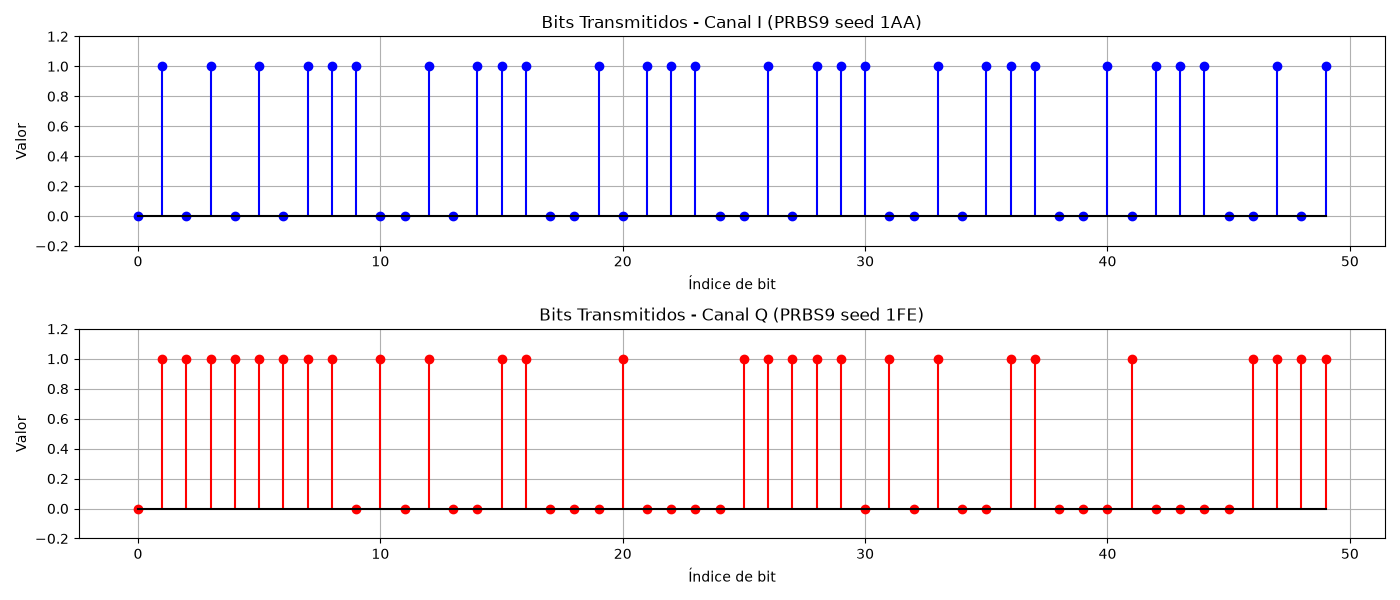
\includegraphics[width=0.85\textwidth]{../images/bits_transmitidos.png}
    \caption{Bits transmitidos por el generador PRBS9 para las componentes I y Q.}
\end{figure}

\subsubsection{Respuesta al impulso y frecuencia del filtro TX}

En la figura se presenta la respuesta al impulso del filtro Raised Cosine con
$\beta = 0.5$. Se observa la forma característica de sinc ponderada por una
cosenoidal en el dominio temporal, con un pico central y lóbulos laterales que
decaen rápidamente. La duración total del filtro es de $N_{baud} = 8$ símbolos
($32$ muestras con $OS = 4$).

\begin{figure}[H]
    \centering
    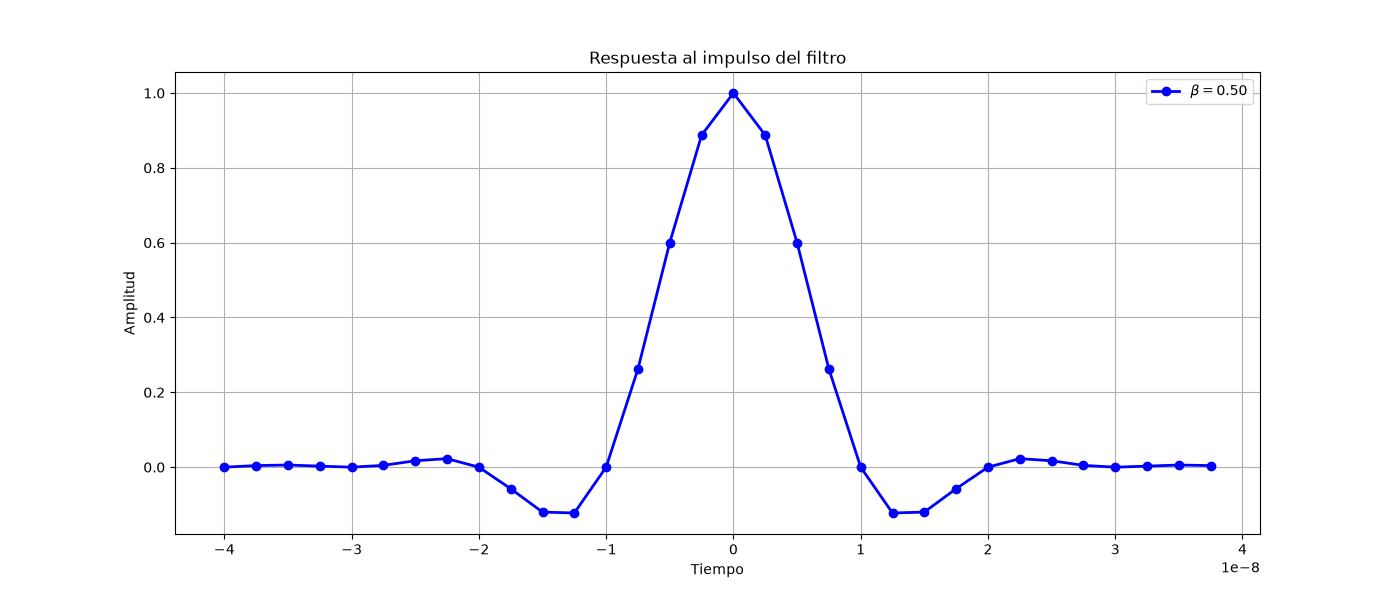
\includegraphics[width=0.85\textwidth]{../images/impulso.png}
    \caption{Respuesta al impulso del filtro Raised Cosine con $\beta = 0.5$.}
\end{figure}

En la Figura de abajo se muestra la respuesta en frecuencia del filtro. Puede
observarse la banda de transición que se extiende desde $50$\,MHz hasta
$75$\,MHz. La caída en la banda de transición es suave debido al valor de
$\beta = 0.5$, y se marca con una línea punteada el nivel de $-6$\,dB que
corresponde al punto de corte del roll-off.

\begin{figure}[H]
    \centering
    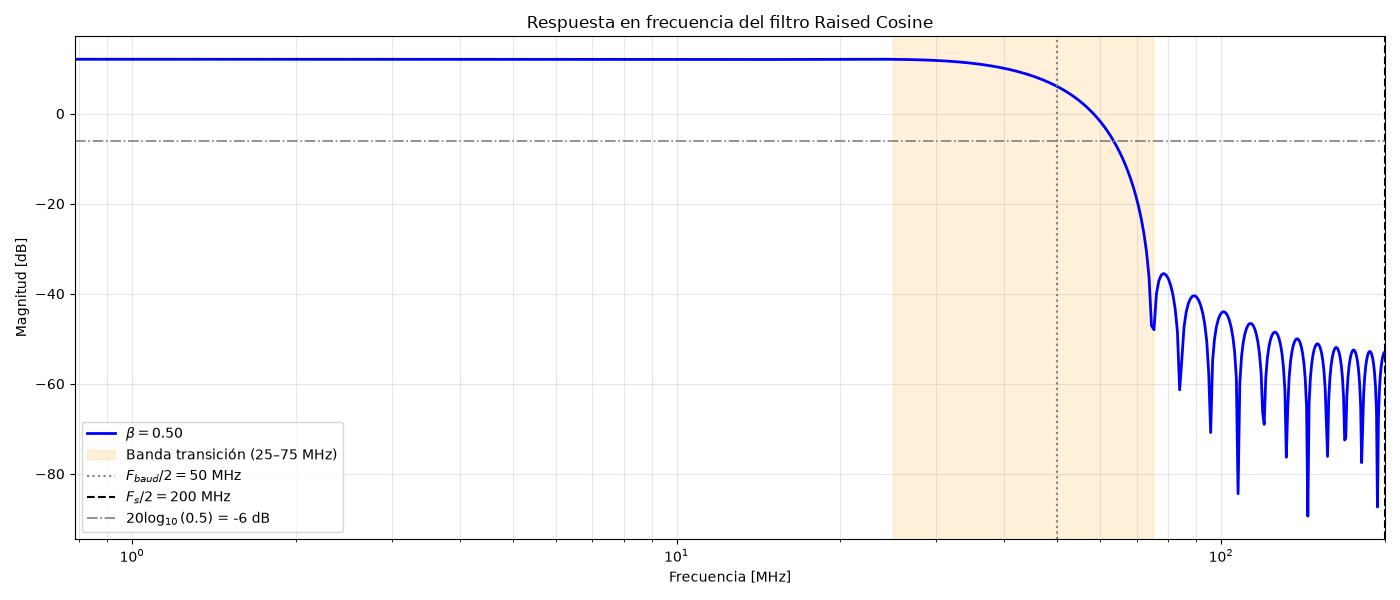
\includegraphics[width=0.85\textwidth]{../images/frecuencia.png}
    \caption{Respuesta en frecuencia del filtro Raised Cosine con $\beta = 0.5$.}
\end{figure}

\subsubsection{Salida y Diagrama de Ojo del filtro TX}

En la figura se muestra la señal filtrada para las componentes I y Q. Se
observa la forma de onda continua, resultante de la convolución entre los
símbolos interpolados y el pulso Raised Cosine. Las transiciones entre símbolos
son suaves, producto del filtrado, y la señal mantiene una envolvente
controlada.

\begin{figure}[H]
    \centering
    
\includegraphics[width=0.85\textwidth]{../images/salida_filtro.png}
    \caption{Señal filtrada a la salida del filtro TX para las componentes I
        y Q.}
\end{figure}

En la siguiente figura se presentan los diagramas de ojo para las componentes I
y Q. Para esta simulación se encontró el offset de muestreo óptimo de manera
empírica, dando como resultado un offset de 1 donde el periodo de muestreo
coincide con el pico de la respuesta al impulso del filtro.

\begin{figure}[H]
    \centering
    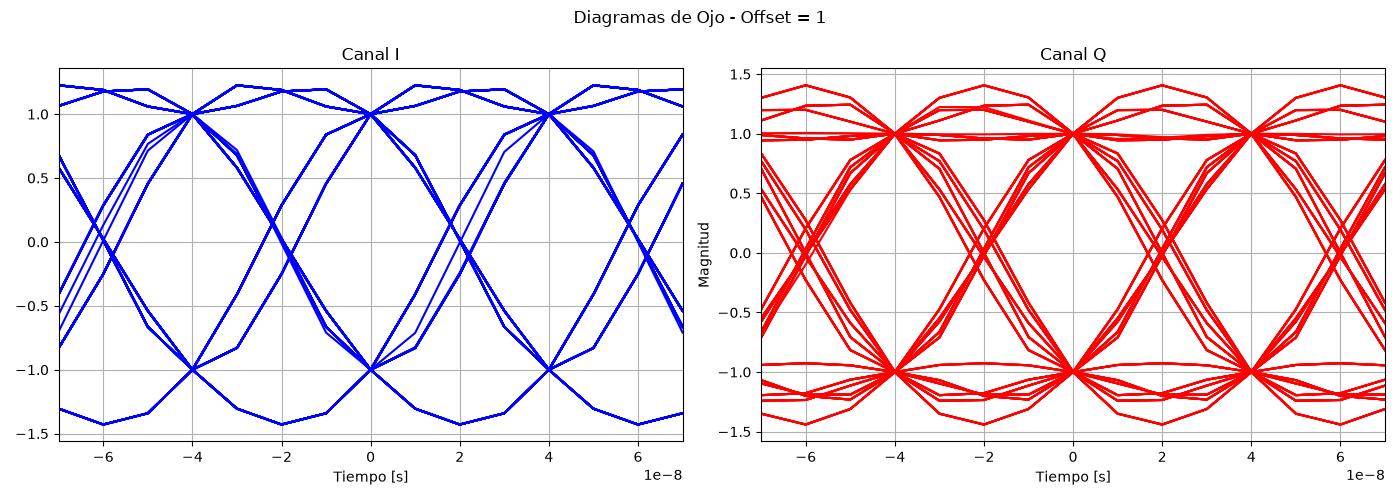
\includegraphics[width=0.9\textwidth]{../images/diagrama_ojo.png}
    \caption{Diagramas de ojo de las componentes I (azul) y Q (rojo).}
\end{figure}

\subsubsection{Diagrama de constelación a la salida del filtro TX}

A continuación se compara la constelación a la salida del filtro TX para las
cuatro fases de muestreo posibles con $OS = 4$: fase 0, 1, 2 y 3. Esta
comparación permite visualizar cómo la selección del offset de muestreo afecta
directamente la calidad de la constelación.

\begin{figure}[H]
    \centering
    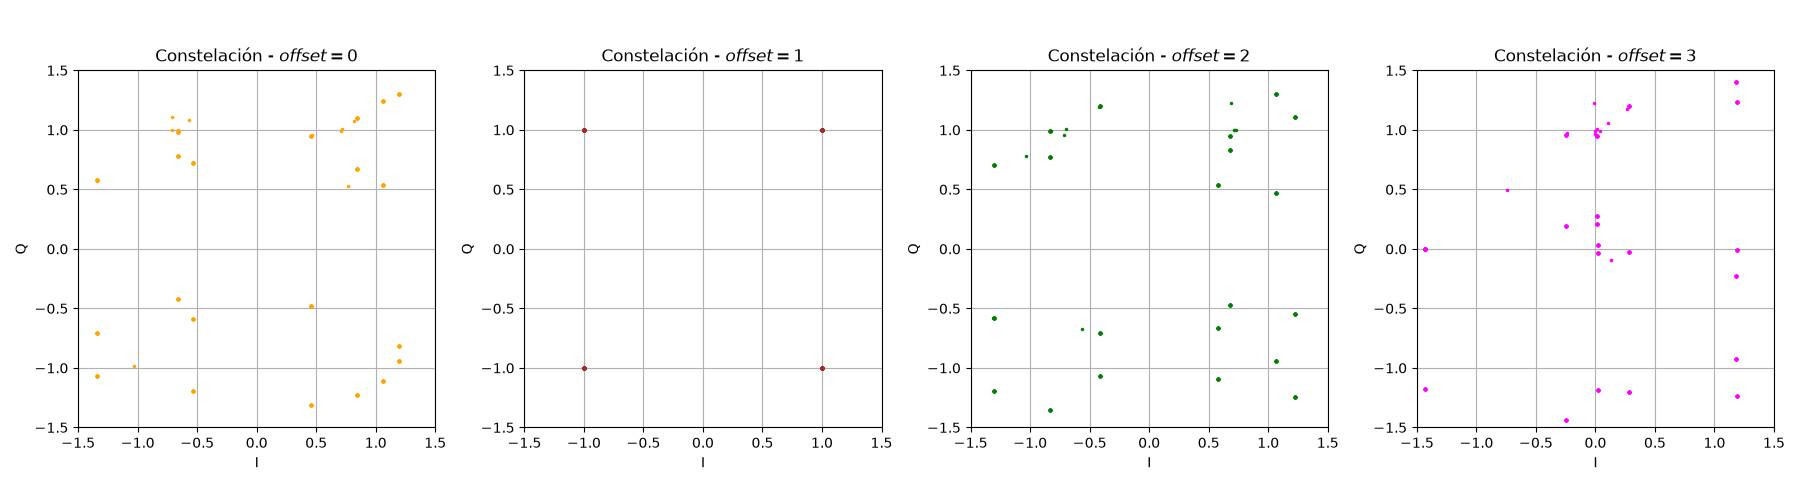
\includegraphics[width=0.95\textwidth]{../images/constelacion.png}
    \caption{Constelación QPSK para las cuatro fases de muestreo.}
\end{figure}

Se observa que la \textbf{fase 1} es la óptima: los 4 puntos QPSK aparecen
perfectamente definidos en las posiciones ideales $(\pm 1, \pm 1j)$, sin
dispersión alguna. Esto confirma que en este punto la propiedad de ISI nula del
filtro Raised Cosine se cumple exactamente.

Las fases 0, 2 y 3 presentan distintos grados de dispersión, indicando que el
muestreo no se realiza en el punto de ISI nulo.

\subsubsection{Bit Error Rate (BER)}

Se calculó la BER comparando los bits transmitidos con los bits recibidos
(muestreados en la fase óptima y decodificados con umbral en cero). En el
escenario de loopback sin ruido, la BER obtenida para el offset óptimo fue de
$0.0 \%$ para ambos canales, confirmando que el sistema de transmisión funciona
correctamente.

\begin{figure}[H]
    \centering
    \begin{lstlisting}[frame=single, basicstyle=\scriptsize\ttfamily]
    Bit Error Rate (BER) Results: (offset = 1)
    BER Canal I: 0.00 % (Errores: 0/511)
    BER Canal Q: 0.00 % (Errores: 0/511)
\end{lstlisting}
    \caption{Resultados de BER para el offset optimo.}
\end{figure}

Tambien se comprobaron los resultados de BER para los offsets no óptimos, en
los casos de offset 0 y 2 se mantuvo el BER en 0.0\%, mientras que para el
offset 3 se obtuvo un BER de 0.28\% para ambos canales, indicando que una
selección incorrecta del offset de muestreo puede introducir errores en la
decodificación de los bits.

\begin{figure}[H]
    \centering
    \begin{lstlisting}[frame=single, basicstyle=\scriptsize\ttfamily]
    Bit Error Rate (BER) Results: (offset = 3)
    BER Canal I: 0.28 % (Errores: 147/511)
    BER Canal Q: 0.28 % (Errores: 144/511)
\end{lstlisting}
    \caption{Resultados de BER para el offset no óptimo.}
\end{figure}

\subsection{Fase 2: Simulación en Python de Punto Fijo}

\section{Conclusiones}

\end{document}
